% siminos/spatiotemp/chapter/reversal.tex
% $Author: predrag $ $Date: 2021-09-15 01:14:55 -0400 (Wed, 15 Sep 2021) $

\section{Time reversal symmetry reduction}
\label{sect:reversal}
\renewcommand{\ssp}{\ensuremath{\phi}}             % lattice site field
\renewcommand{\Ssym}[1]{{\ensuremath{m_{#1}}}}    % Boris
\renewcommand{\Xx}{\ensuremath{\mathsf{\Phi}}}      % kittens lattice field


\subsection{Laplacians (and time reversal?)}
\label{sect:LapReversal}

                                                    \toCB
%   \item[2020-10-31 Predrag]

The symmetric (self-adjoint) Laplacian
$\Box = - \transp{\partial}\partial$
suggests that time-reversal desymmetrized dynamics is given by a first
order derivative \(
\partial = \shift  - \unit
\)
(also known as the integer lattice forward difference operator, see \refeq{forwDer},
\refeq{Elaydi05(2.1.1)}).
The symmetric (self-adjoint) combination
$\Box = - \transp{\partial}\partial$ % = \partial^2$
is the Laplacian
\index{lattice!Laplacian}\index{Laplacian!lattice}
\bea
\jMorb &=&  \Box - {\mu}^2\unit
       \,=\, -
  \left(\shift^{-1}  - \unit \right)
  \left(\shift       - \unit \right)
   - {\mu}^2\unit
\,,
\label{LatLap}
\eea
where
\beq
{\mu }= \sqrt{s-2}
\,.
\ee{templattMass}
is the
Yukawa mass parameter \refeq{catlattMass} in $d=1$ dimension.

For purposes of the time-reversal desymmetrization its is
more convenient to work with the centered,
reflection antisymmetric difference operators \refeq{Box(2.1.1)},
\bea
\tilde{\partial} &=&
\tilde{\shift}-\tilde{\shift}^{-1}
\,,\qquad
\tilde{\shift}=\shift^{1/2}
    \continue
 &=& - \transp{\tilde{\partial}}
\,,
\label{centeredDiffOper}
\eea
constructed by interpolating 1/2-unit spacing lattice $\tilde{\lattice}$
points between the integer lattice \lattice\ points, with the derivatives
written as
\bea
\left(\shift-\unit\right)
 &=&
\tilde{\shift}\tilde{\partial}
     % \left(\tilde{\shift}-\tilde{\shift}^{-1}\right)
    \continue
\left(\shift^{-1}-\unit\right)\left(\shift-\unit\right)
 &=&
    - \tilde{\partial}^2
  = \Box
    %\left(\tilde{\shift}-\tilde{\shift}^{-1}\right)^2
 \label{Lat-LapSqrt}\\
\jMorb  &=& \Box - \mu^2\unit
         = \transp{\tilde{\jMorb}}\tilde{\jMorb}
%\left(
%\tilde{\partial} + \mu\unit  %\left(\tilde{\shift}-\tilde{\shift}^{-1}\right)
%\right)
%\left(
%\tilde{\partial} - \mu\unit  %\left(\tilde{\shift}-\tilde{\shift}^{-1}\right)
%\right)
    \continue
\tilde{\jMorb}
     &=& \tilde{\partial} - {\mu}\unit
    \,=\,
    \tilde{\shift} - \mu\unit -\tilde{\shift}^{-1}
    \continue
\transp{\tilde{\jMorb}}
     &=& \tilde{\partial} + {\mu}\unit
    \,=\,
    \tilde{\shift} + \mu\unit -\tilde{\shift}^{-1}
\nnu
\eea
Written out in the matrix form, the
$\jMorb=\transp{\tilde{\jMorb}}\tilde{\jMorb}$ factorization
can be checked by matrix multiplication
    \PC{2021-09-14}{
    Checked that factorization \refeq{tildejMorb}, metal temporal lattice
    condition \refeq{GoldenCatRec} works also for the orbit $\Xx$
    dependent case \refeq{jMorb1dFT}.
    }
\bea
\jMorb[\Xx]
  &=&
\left(
\begin{array}{ccccccc}
-{s}_{0}& 0 & {1} & 0 & \dots & {1} & 0 \\
 0 &-{s}_{1}& 0 & {1} & \dots & 0 & {1} \\
 {1} & 0 &-{s}_{2}& 0 & \dots & 0 & 0 \\
 \vdots & \vdots & \vdots & \ddots & \vdots & \vdots & \vdots \\
 0 & 0 & \dots & 0 &-{s}_{\cl{}-3}& 0 & {1} \\
 {1} & 0 & \dots & {1} & 0 &-{s}_{\cl{}-2}& 0 \\
 0 & {1} & \dots & 0 & {1} & 0 &-{s}_{\cl{}-1}\\
\end{array}
\right)
    \continue
\tilde{\jMorb}
  &=&
\left(\begin{array}{ccccccc}
-\mu_{0} &{-1}  & 0 & 0 &\dots &0& 1\\
 1   &-\mu_{1} &{-1}& 0 &\dots &0&0 \\
 0 &  1 &-\mu_{2} &{-1}&\dots &0 & 0 \\
\vdots & \vdots &\vdots & \vdots & \ddots &\vdots &\vdots\\
 0 & 0 & \dots &\dots &\dots  &-\mu_{\cl{}-2}&{-1}\\
{-1}& 0 & \dots &  \dots &\dots& 1 &-\mu_{\cl{}-1}
        \end{array} \right)
\,,
\label{tildejMorb}  % copy of PC(1.2.11)}
\eea
where
$\mu_{\zeit}^2={s}_{\zeit}-2$ is the lattice site "Klein-Gordon mass",
"stretching factor", respectively,
and
$\jMorb, \transp{\tilde{\jMorb}}, \tilde{\jMorb}$ act on the 1/2-unit
spacing lattice $\tilde{\lattice}$, \ie,  remember
    \PCedit{
(perhaps reintroduce $\Delta\zeit$ lattice spacing explicitly?)
    }
that $\tilde{\shift}=\shift^{1/2}$ in \refeq{Lat-LapSqrt} is the shift
operator on the 1/2 lattice spacing. So two applications of 1/2 lattice
shift operator give you one full lattice spacing.

%    \item[2020-02-06 Predrag]
Written out as a second-order difference equation, the metal map
takes a temporal lattice form
\beq
\tilde{\ssp}_{\zeit+1}  -  \mu{_\zeit}\tilde{\ssp}_{\zeit} - \tilde{\ssp}_{\zeit-1}
    =
-\tilde{\Ssym{\zeit}}
\,,
\ee{GoldenCatRec}
or,
in terms of a {{\lattstate}} $\Xx$, the corresponding {symbol \brick}'
$\Mm$, and the $[\cl{}\!\times\!\cl{}]$ {\shiftOp}
$\shift$, % \refeq{hopMatrix},
\beq
(\tilde{\shift} - \mu[\Xx]\id - \tilde{\shift}^{-1})\,\tilde{\Xx} = -\tilde{\Mm}
\,,
\ee{catTempLatt}
where $\mu[\Xx]\id$ stands for site-dependent diagonal Klein-Gordon mass matrix.

$\tilde{\jMorb}$ discrete
Fourier diagonalization
\bea
\lambda_m &=& {\mu}^2+2-2\cos\alpha_m = {\mu}^2+ 4 \sin^2\left(\alpha_m/2\right)
\continue
   &=& \left({\mu} - i\,2\sin\left(\frac{\alpha_m}{2}\right)\right)
   \,  \left({\mu} + i\,2\sin\left(\frac{\alpha_m}{2}\right)\right)
\continue
   &=& \left({\mu} + \e^{i\alpha_m/2}-\e^{-i\alpha_m/2}\right)
   \,  \left({\mu} + \e^{i\alpha_m/2}-\e^{-i\alpha_m/2}\right)^*
\continue
&&\qquad\mbox{where }\quad \alpha_m \,=\, 2\pi{m}/{n}
\label{tildejMorbDisg} % copied from Pozrikidis14(1.2.7a)}
\eea
\ie, the
$\sin^2\left(\alpha_m/2\right)$ version of the eigenvalues
is there for a reason, a consequence of the time-reversal symmetry,
with $\tilde{\jMorb}$ eigenvalues being
\[
-2i\sin\left(\alpha_m/2\right)= \e^{i\alpha_m/2}-\e^{-i\alpha_m/2}
\,.
\]
Phase is $\alpha_m/2$ because the fundamental domain is
1/2 of the full line.
The square root is natural because the Yukawa mass ${\mu}^2=d(s-2)$
parameter \refeq{catlattMass}.

Discrete Fourier diagonalization
\(
\jMorb=\jMorb_{-}\jMorb_{+}
\,,
\)
 turns $\tilde{\shift}$ into its
eigenvalues $\exp(i\alpha_k/2)$, and the \templatt\ {\HillDet}
\refeq{HL:detTemCatCheb} factorizes as
\bea
\Det\jMorb  &=& \Det\jMorb_{-}\,\Det\jMorb_{+}
    \continue
\Det \jMorb_{+}
 &=& {\mu}\prod_{k=1}^{\period{}-1}
         ({\mu}+2 i \sin(\alpha_k/2))
    \,,\qquad
 \alpha_k =2 \pi{k}/\period{}
    \continue
\Det \jMorb_{-}
 &=& {\mu}\prod_{k=1}^{\period{}-1}
         ({\mu}-2 i \sin(\alpha_k/2))
\,.
\label{PC:detTemFact}
\eea

By derivation \PCedit{(do it!)} analogous to the Isola's
cat map  ${\zeta}(Z)$ \refeq{Isola90-13b},
the topological zeta function for metal cat maps is
\beq
\frac{1}{\tilde{\zeta}(t)}
%           = \frac{(1 - \Lambda t) (1 - \Lambda^{-1} t)}
%                 {(1 - t)^2}
           =  \frac{1 - \mu t - t^2}
                  {(1 - t)^2}
 \,,
\ee{metalZeta}
where $z=t^2$,
in agreement with \refeq{AABHM99-46a} for $\mu=1$.
See also \refeq{Wilf94:FibRecGF}.

%What is this square root of $z$? This is expected, see
%\toChaosBook{section.25.5}
%{sect.~25.5} {\em $\Zn{2} = \Dn{1}$ factorization}:
%[...]
%if a cycle
%${p}$ is invariant under the symmetry subgroup ${\cal H}_{{p}} \subseteq G$ of
%order $h_{{p}}$, its weight can be written as a repetition of a fundamental
%domain cycle
%\beq
%t_{{p}} =  t_{\hat{p}}^{ h_{{p}} }
%\label{t-power}
%\eeq
%computed on the irreducible segment that corresponds to a
%fundamental domain cycle. [...] In the $\Dn{1}$ case, $t_{{p}}$
%is a {\orbit}, or
%a double repeat of a {\orbit}, $t_{{p}} =  t_{\hat{p}}^2$,
%hence the square root.

%    \item[2021-02-12 Han]
Denote the $[\tilde{n}\times\tilde{n}]$ {\jacobianOrb}
$\tilde{\jMorb}(\mu)$ of the 1/2 time-step lattice $\tilde{\lattice}$ as
$\tilde{\jMorb}_{\tilde{n}}$, where $\tilde{n}$ is the period of the
{\lattstate}  $\tilde{\Xx}$ on the half interval lattice
$\tilde{\lattice}$.
Denote the {\jacobianOrb} ${\jMorb({s})}$ of the \templatt\ lattice
${\lattice}$  as ${\jMorb}_n$, where $n$ is the period of the {\lattstate} $\Xx$ on the integer lattice ${\lattice}$. For odd, respectively
even periods, the determinants of $\tilde{\jMorb}$ and ${\jMorb}$ are
related as:
\bea
\det(\transp{\tilde{\jMorb}}_{2m+1}\tilde{\jMorb}_{2m+1})
&=& \det({\jMorb}_{2m+1})
    \continue
\det(\transp{\tilde{\jMorb}}_{2n}\tilde{\jMorb}_{2n})
&=& \det({\jMorb}_{n})^2 \,,
\label{tildejMorbRelation}
\eea
hence
    \PC{2021-02-13}{
    Have not checked whether absolute values $|\cdots|$ are needed for
    the even case.
    }
\bea
{N}(s)_{\cl{}} &=& \det{\jMorb}_{n}
    =
(\det\tilde{\jMorb}_{n})^2 = \tilde{N}(\mu)_{\cl{}}^2
    \,,\quad
n \mbox{ odd}
    \continue
{N}(s)_{\cl{}} &=& |\det{\jMorb}_{n}|
    =
|\det\tilde{\jMorb}_{2n}| =  \tilde{N}(\mu)_{2\cl{}}
    \,,\quad
n \mbox{ even}
\,.
\label{tildejMorbRel}
\eea
For odd $n$, see
\refeq{catFundPar3} and compare odd entries in \reftab{tab:catMapN_n-s=3}
and \reftab{BaRoWe08fib-tab}.

For even $n$, compare the
$n$ entries in \reftab{tab:catMapN_n-s=3}
with the $\tilde{n}=2n$ entries in \reftab{BaRoWe08fib-tab}.

%%%%%%%%%%%%%%%%%%%%%%%%%%%%%%%%%%%%%%%%%%%%%%%%%%%%
\begin{table}
\begin{tabular}{c|rrrrr|rrrrr|rrrrr}
$\cl{}$ &  1 &  2 &  3 &  4 &  5 &
       6 &  7 &  8 &  9 & 10 &
      11 \\%& 12 & 13 & 14 & 15 \\
\hline
$N_\cl{}$ &   1 &   5 &  16 &  45 &  121 &
        320 & 841 & 2205 &5776 &15125&
       39601& %   &      &     & 1364
             \rule[-1ex]{0ex}{3.5ex} \\
$M_\cl{}$ &   1 &   2 &   5 &  10 &   24 &
         50 & 120 & 270 & 640 & 1500 &
       3600 &  %% &     &     &
\end{tabular}
\bigskip
\caption{\label{tab:catMapN_n-s=3}
{\Lattstate}s and %{prime}
orbit counts for the ${s}=3$ cat map.
Compare with the golden (Fibonacci\rf{BaNeRo13}) cat map
\reftab{BaRoWe08fib-tab} and \refeq{zetasqrt-N}.
}
\end{table}
%%%%%%%%%%%%%%%%%%%%%%%%%%%%%%%%%%%%%%%%%%%%%%%%%%%%
%

%%%%%%%%%%%%%%%%%%%%%%%%%%%%%%%%%%%%%%%%%%%%%%%%%%%%
\begin{table}
\begin{tabular}{c|rrrrr|rrrrr|rrrrr}
$\cl{}$ &  1 &  2 &  3 &  4 &  5 &
       6 &  7 &  8 &  9 & 10 &
      11 & 12 & 13 & 14 & 15 \\
\hline
$\tilde{N}_\cl{}$ &   1 &   1 &   4 &   5 &   11 &
         16 &  29 &  45 &  76 &  121 &
        199 & 320 & 521 & 841 & 1364\rule[-1ex]{0ex}{3.5ex} \\
$\tilde{M}_\cl{}$ &   1 &   0 &   1 &   1 &    2 &
          2 &   4 &   5 &   8 &   11 &
         18 &  25 &  40 &  58 &   90
\end{tabular}
\bigskip
\caption{\label{BaRoWe08fib-tab}
    Temporal {\lattstate}s and {\orbit} counts for the
    $\mu=1$  golden cat map.
    See \refeq{zetasqrt-N} and the counting of walks on
    the ``half time-step'' Markov graph \reffig{fig:HLHalfStepMarkov}.
    }
\end{table}
%%%%%%%%%%%%%%%%%%%%%%%%%%%%%%%%%%%%%%%%%%%%%%%%%%%%


$\hat{\jMorb}=\transp{\tilde{\jMorb}}\tilde{\jMorb}$ is the {\jacobianOrb}
of the \templatt\ on the half interval lattice $\tilde{\lattice}$
(denoted $\jMorb$ in \refeq{tildejMorb}).
$\hat{\jMorb}_{2n}=\transp{\tilde{\jMorb}}_{2n}\tilde{\jMorb}_{2n}$
is the {\jacobianOrb} of the \templatt\ on the half lattice with period $2n$,
which is period $n$ in the unit lattice. But $\hat{\jMorb}_{2n}$
is different from ${\jMorb}_{n}$, the {\jacobianOrb} of the \templatt\ on the unit lattice,
because it has more lattice sites. Note that:
\[
\hat{\jMorb}_{2n} = {\jMorb}_{n} \otimes \unit_{[2 \times 2]} \, .
\]
Using the second identity in \refeq{wikiKron2} we can get the second relation in
\refeq{tildejMorbRelation}.

$\hat{\jMorb}_{2n+1}=\transp{\tilde{\jMorb}}_{2n+1}\tilde{\jMorb}_{2n+1}$ is the
{\jacobianOrb} of the \templatt\ on the half lattice with period $2n+1$,
which has period $n+1/2$ on the unit lattice. $\hat{\jMorb}_{2n+1}$ is same as the
${\jMorb}_{2n+1}$ after a permutation, which leads to the first relation in
\refeq{tildejMorbRelation}.

%    \item[2016-11-16 Predrag]
The ``functional equation''\rf{AnBoMa99} % of Angl{\`e}s d'Auriac \etal
\beq
\zeta(z)=\zeta(1/z)
\ee{templattZetaFctEq} % copied from {AnBoMa99-3.22a}
is for us the obvious statement of time-reversal invariance.
Note also under the time reversal $t\to1/t$
\beq
\frac{1}{\tilde{\zeta}(1/t)}  = -\,\frac{1}{\tilde{\zeta}(-t)}
\,.
\ee{timeRevZeta}    % copy of{timeRevPC}


\subsection{Time reversal blog}
\label{sect:reverseBlog}

\begin{description}

%%%%%%%%%%%%%%%%%%%%%%%%%%%%%%%%%%%%%%%%%%%%%%%%%%%%%%%%%%%%
% figs from y-lan/ks/figs/              2004-11-01
\begin{figure}% [tbp] %[h]
    \centering
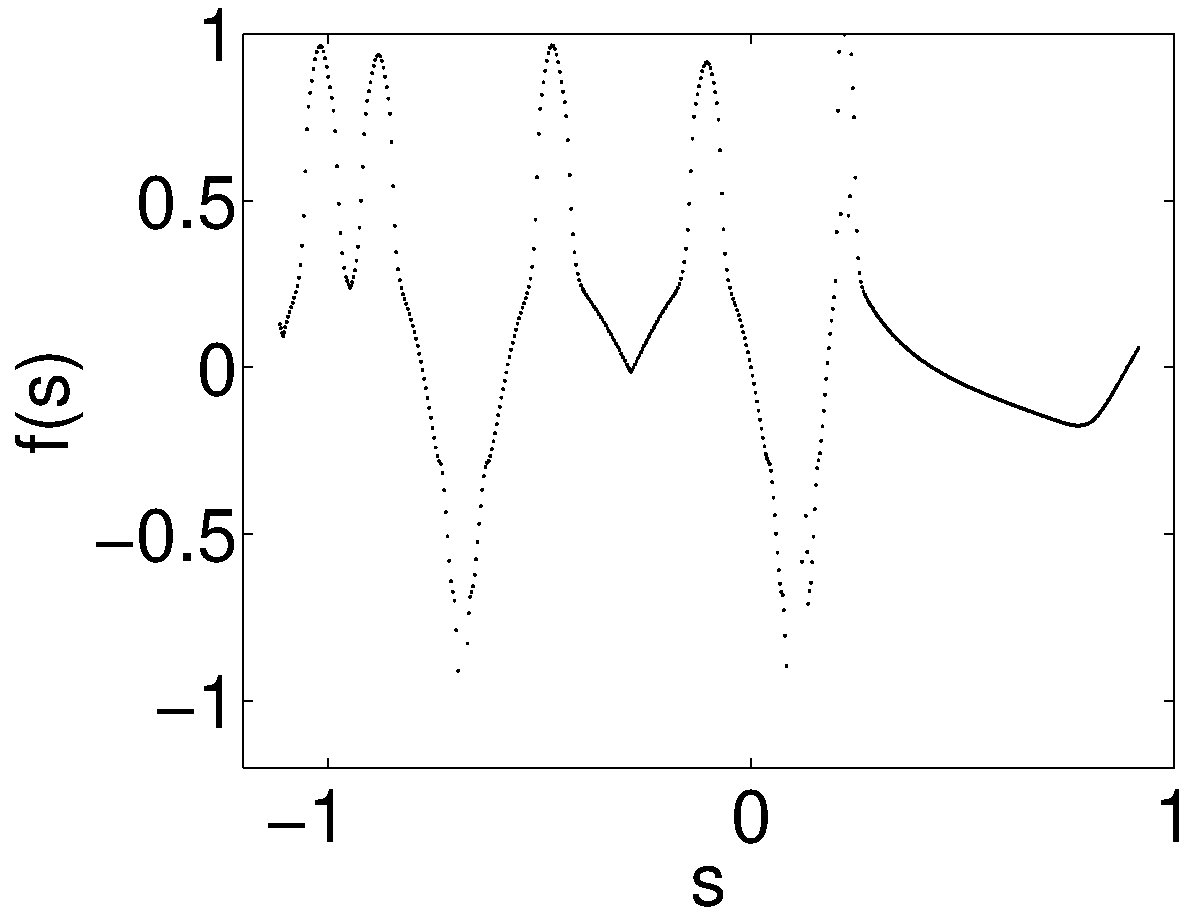
\includegraphics[width=0.74\textwidth]{antmp1}
\\
\hspace{0.10\textwidth}
(a)
\\
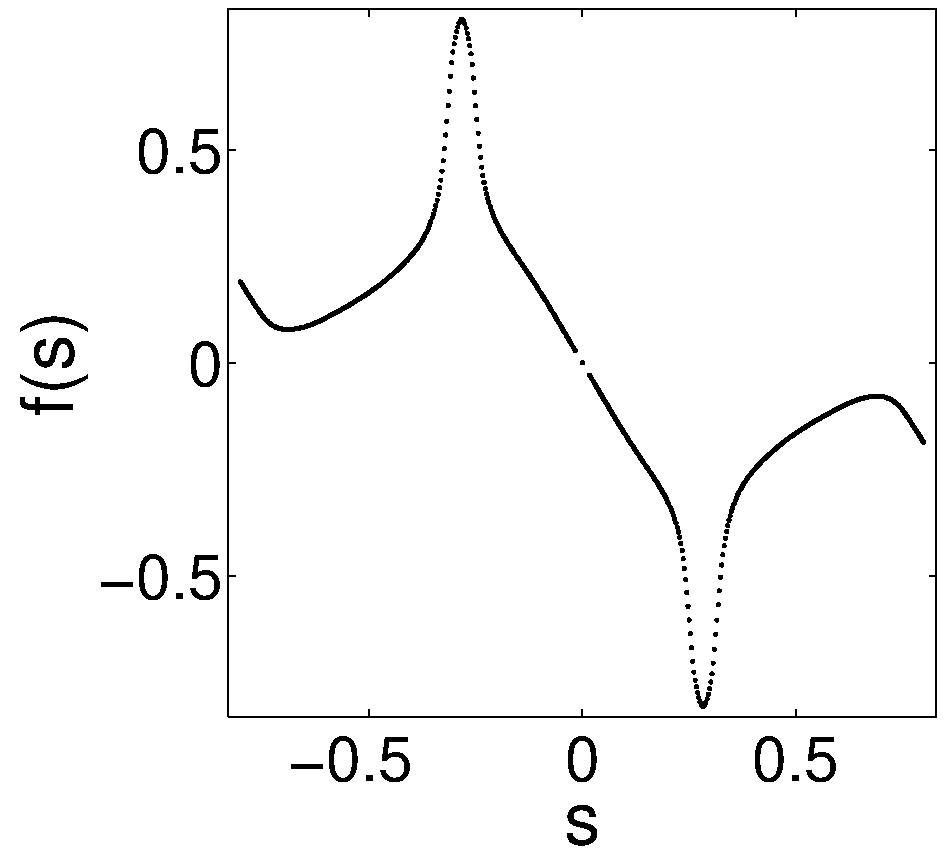
\includegraphics[width=0.44\textwidth]{ant5mmp}
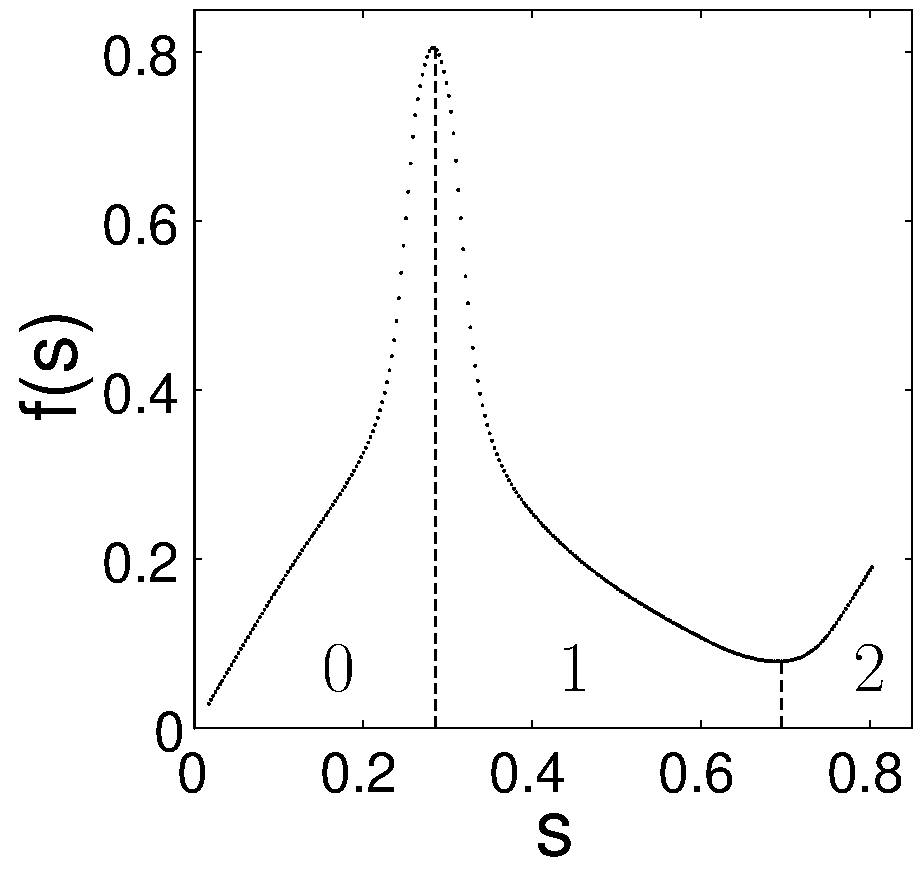
\includegraphics[width=0.44\textwidth]{ant5mmpf}
\\
\hspace{0.10\textwidth}(b)\hspace{0.44\textwidth}(c)
\caption[]{
The \PoincMap\ on the \PoincSec\ $\mathcal{P}_C$ of the
unstable manifold of \eqv\ $C$, antisymmetric subspace of \KS, the
intrinsic coordinate:
(a) There are 11 monotone segments, requiring an 11-letter alphabet.
However, in the (\KS)/{\Dn{1}}-spatial reflection symmetry reduced
\statesp,
(b)
the \PoincMap\ simplifies to an antisymmetric return map,
which becomes
(c)
a 3-letter bimodal return map in the fundamental domain, with the
symbolic dynamics given by three symbols $\{0\,,1\,,2\}$.
It's a \textbf{wild} $\sqrt{\mbox{time}}$ simplification of the dynamics!
enabling us to populate the neighboring strange attractor with
many periodic orbits.
(Taken from fig.~8\,(e) of Lan and Cvitanovi\'c\rf{lanCvit07}).
      }
\label{f:antmn1}
\end{figure}
%%%%%%%%%%%%%%%%%%%%%%%%%%%%%%%%%%%%%%%%%%%%%%%%%%%%%%%%%%%%

    \item[2007-11-20 Keating,  Marklof and Williams]
% doi:10.1088/1367-2630/10/8/083023
The cat map $A$ acting on $(q_\zeit,p_\zeit)$  must be symplectic, and
time-reversal symmetric,
\beq
T A T=A^{-1}
\ee{KeMaWi07(8)}
where $T$ is the time-reversal operator
\beq
T=
\MatrixII{1}{0}
         {0}{-1}
\ee{KeMaWi07(9)}
An example is
% http://shiftleft.com/mirrors/www.hpl.hp.com/techreports/98/HPL-BRIMS-98-07.pdf
% T.O.deCarvalho*,J.P.Keatingi-,J.M.Robbinst
\beq
A=
\MatrixII{2}{1}
         {3}{2}
\ee{CaKero98(9)}
The \PV\ 2-configuration map \refeq{PerViv:2confRepMat}
acts on a 2\dmn\ \statesp\ point $(\ssp_{n-1},\ssp_{n})$,
so time reversal permutes the two entries,
\beq
A=
\MatrixII{0}{1}
         {-1}{s}
\,,\qquad
T=
\MatrixII{0}{1}
         {1}{0}
\,.
\ee{PerViv:2confRepMat1}
Not sure what $T$ is for cat map of form \refeq{eq:CatMapIntr}.


    \item[2004-11-01 Predrag and Lan]
We implemented the ``half-step'' \reffig{fig:HLHalfStepMarkov} reduction
for the \KS\ spatial reflection symmetry in
\HREF{http://chaosbook.org/~predrag/papers/preprints.html\#ks} {\em
Unstable recurrent patterns in Kuramoto-Sivashinsky
dynamics}\rf{lanCvit07}, see \reffig{f:antmn1}.
It happens in sect.~B {\em Curvilinear coordinates, center repeller} of
the paper, and the result is the 3-letter bimodal return map of
\reffig{f:antmn1}\,(c). Without quotienting the $\Dn{1}$ symmetry, the
return map would have up to 11 letters, and be an unmaneagable holly mess.

    \PCpost{2018-04-12}{
For our many (failed) attempts to find an \AW\ forward and
backward in time symmetric partition, see \refsect{sect:timeRev} {\em
Time reversal}.
    }

    \PCpost{2018-04-12}{
\HREF{http://birdtracks.eu/courses/PHYS-7143-19/notes.pdf\#subsection.8.2.3}
{Birdtracks.eu Sect.~8.2.3} {\em  Time reversal symmetry} might be
relevant to \catlatt: when the Hamiltonian is invariant under time
reversal, the symmetry group is enlarged.
    }

    \item[2016-11-16 Predrag]
Maillard group,
Angl{\`e}s d'Auriac, Boukraa and Maillard\rf{AnBoMa99}
{\em Functional relations in lattice statistical mechanics, enumerative
combinatorics, and discrete dynamical systems}
state the ``functional equation''
\beq
\zeta(z)=\zeta(1/z)
\ee{AnBoMa99-3.22a}
which for us is the obvious statement of time-reversal invariance.

    \item[2016-11-16 Predrag]
Note also \refeq{timeRevZeta} under the presumed time reversal $t\to1/t$
%\beq
%\frac{1}{\tilde{\zeta}(1/t)}
%    = -\frac{1}{\tilde{\zeta}(-t)}
%\,.
%\ee{timeRevPC}
This all has to do with time reversibility - we should exploit time and space
reversal symmetries in this way, and - who knows - understand Ihara zeta
functions better.
% It also reminds me of the discrete symmetry factorizations
% of zeta's in ChaosBook.org.

%    \item[2021-01-30 ERROR]
%    Given `square-root' zeta function \refeq{AABHM99-46}
%\beq
%\frac{1}{\tilde{\zeta}(t)}
%    =  \frac{1 - t - t^2}
%            {(1 - t)^2}
%\,,
%\ee{AABHM99-46a}
%$N_n$, the number of \emph{{\lattstate}s} of period $n$ is given by the
%logarithmic derivative of the `square-root' zeta function
%\refeq{zetatop-N},
%\bea
%\sum_{n=1}N_n t^n
%    &=& - \,\frac{1}{\tilde{\zeta}} t \frac{d}{dt} \frac{1}{\tilde{\zeta}}
%\continue
%    &=& -t +  t^2 +2\,t^3 +5\,t^4 +9\,t^5 +16\,t^6 +27\,t^7
%    \ceq
%    +45\,t^8 +74\,t^9 +121\,t^{10} +1971\,t^{11}
%    + \dots
%\,.
%\label{zetasqrt-N}
%\eea


    \item[2020-12-24 Predrag]
Note that in the discussion of time-reversal invariant recurrence
relations \refeq{FGHLW74:charFunct1d} (see \refeq{3diagToeplitz}, \etc)
the characteristic equation factors as $a(\ssp)=\ell(\ssp)\,\ell(l/\ssp)$
where the factors $\ell(\ssp)$ and $\ell(l/\ssp)$ of $a(\ssp)$ are known
as the \emph{Hurwitz factors}.

    \item[2020-01-10 Predrag]
The ``square root'' $C$ \refeq{AABHM99-44} might be related to resistor
networks's Laplace-like operator factorization $L = R\transp{R}$, see
\refeq{Pozrikidis14(1.1.6)}, with no transpose needed in this
example, as $C$ is
symmetric.

%A wild
%$\jMorb=\transp{\tilde{\jMorb}}\tilde{\jMorb}$
%factorization guess, \PCedit{clearly wrong} (works only
%for $s=2$):
%\beq
%\jMorb
%  =
%\left(\begin{array}{ccccccc}
%  {s}&{-1}& 0 & 0 &\dots &0&{-1}\\
%{-1}&   {s}&{-1}& 0 &\dots &0&0 \\
%0 &{-1}&   {s}&{-1}&\dots &0 & 0 \\
%\vdots & \vdots &\vdots & \vdots & \ddots &\vdots &\vdots\\
%0 & 0 & \dots &\dots &\dots  &  {s}&{-1}\\
%{-1}& 0 & \dots &  \dots &\dots&{-1}&   {s}
%        \end{array} \right)
%\,.
%\ee{Pozrikidis14(1.2.10)}
%
%\beq
%\tilde{\jMorb}
%  =
%\left(\begin{array}{ccccccc}
% {1}&{-1}& 0 & 0 &\dots &0& 0\\
% 0 &  {1}&{-1}& 0 &\dots &0&0 \\
% 0 &  0 &  {1}&{-1}&\dots &0 & 0 \\
%\vdots & \vdots &\vdots & \vdots & \ddots &\vdots &\vdots\\
% 0 & 0 & \dots &\dots &\dots  & {1}&{-1}\\
%{-1}& 0 & \dots &  \dots &\dots& 0 &  {1}
%        \end{array} \right)
%\,.
%\ee{Pozrikidis14(1.2.11)}
%
%\beq
%\transp{\tilde{\jMorb}}
%  =
%\left(\begin{array}{ccccccc}
% {1}& 0 & 0 & 0 &\dots &0&{-1}\\
%{-1}&  {1}& 0 & 0 &\dots &0&0 \\
%0 &{-1}&  {1}& 0 &\dots &0 & 0 \\
%\vdots & \vdots &\vdots & \vdots & \ddots &\vdots &\vdots\\
%0 & 0 & \dots &\dots &\dots  & {1}& 0 \\
%0 & 0 & \dots &  \dots &\dots&{-1}&  {1}
%        \end{array} \right)
%\,.
%\ee{Pozrikidis14(1.2.12)}

    \item[2020-02-06 Predrag]
$\jMorb=\transp{\tilde{\jMorb}}\tilde{\jMorb}$ factorization\rf{Pozrikidis14},
% (the $s=3$ or $\mu=1$ guess \refeq{Pozrikidis14(1.2.10)},
% \refeq{Pozrikidis14(1.2.11)} \PCedit{now corrected})
as in
\refeq{sqrtOrbJac}:
\beq
\tilde{\jMorb}
  =
\left(\begin{array}{ccccccc}
 \mu &{-1}  & 0 & 0 &\dots &0& 1\\
 1   &  \mu &{-1}& 0 &\dots &0&0 \\
 0 &  1 &  \mu &{-1}&\dots &0 & 0 \\
\vdots & \vdots &\vdots & \vdots & \ddots &\vdots &\vdots\\
 0 & 0 & \dots &\dots &\dots  & \mu&{-1}\\
{-1}& 0 & \dots &  \dots &\dots& 1 &  \mu
        \end{array} \right)
\,.
\ee{PC(1.2.11)}

\beq
\transp{\tilde{\jMorb}}
  =
\left(\begin{array}{ccccccc}
 \mu& 1 & 0 & 0 &\dots &0&{-1}\\
{-1}&  \mu& 1 & 0 &\dots &0&0 \\
0 &{-1}&  \mu& 1 &\dots &0 & 0 \\
\vdots & \vdots &\vdots & \vdots & \ddots &\vdots &\vdots\\
0 & 0 & \dots &\dots &\dots  & \mu& 1 \\
1 & 0 & \dots &  \dots &\dots&{-1}&  \mu
        \end{array} \right)
\,.
\ee{PC(1.2.12)}
Note that Pozrikidis\rf{Pozrikidis14} $L = R\transp{R}$ factorization
\refeq{Pozrikidis14(1.1.6)} the factors $R$ are bi-diagonal, as in the
forward difference operator \refeq{LatLap}. He does not seem to introduce
1/2 lattice spacing central difference operator \refeq{centeredDiffOper},
and considers only the Helmholtz equation $\mu=0$ case, not our
tri-diagonal map. I do not see our symmetry reduction there...

$\jMorb$ is time reversal \refeq{timeRefl1} invariant (self-adjoint;
Hermitian), $R\jMorb\transp{R}=\jMorb$, but
$\transp{\tilde{\jMorb}}=\tilde{R}\tilde{\jMorb}\transp{\tilde{R}}$ is time reversed, as
a first order derivative should.

%    \item[2020-01-10 Predrag]
%The correct form of $\tilde{\jMorb}$ should agree with the Toeplitz / discrete
%Fourier diagonalization
%\bea
%\lambda_m &=& {\mu}^2+2-2\cos\alpha_m = {\mu}^2+ 4 \sin^2\left(\alpha_m/2\right)
%\continue
%   &=& \left({\mu} - i\,2\sin\left(\frac{\alpha_m}{2}\right)\right)
%   \,  \left({\mu} + i\,2\sin\left(\frac{\alpha_m}{2}\right)\right)
%\continue
%%\,,\quad
%\alpha_m &=& 2\pi{m}/{n}
%\label{Pozrikidis14(1.2.7a)}
%\eea
%\ie, the
%$\sin^2\left(\alpha_m/2\right)$ version of the eigenvalues
%is there for a reason, a consequence of the time-reversal symmetry,
%with $\tilde{\jMorb}$ eigenvalues being
%\[
%-2i\sin\left(\alpha_m/2\right)= \e^{i\alpha_m/2}-\e^{-i\alpha_m/2}
%\,.
%\]
%Phase is $\alpha_m/2$ because the fundamental domain is
%1/2 of the full line.
%The square root is natural because the Yukawa mass ${\mu}^2=d(s-2)$
%parameter \refeq{catlattMass}.

    \item[2020-09-30 Predrag]
Note that in \refeq{AABHM99-46} Maillard \etal\rf{AnBoMa99} quotient the
time reversal (reflection) symmetry for ${s}=3$ \templatt.

The reflection-symmetric operator
\beq
T_{ij} = \sum^d_{\mu=1}
	 [ (\shift^\mu)_{ij} + (\shift^\mu)_{ji}]
	\,,
% \qquad h_\mu = (h,h, \cdots,h)
\label{(5.3)}
\eeq
generates all steps of length 1.
The symmetric (self-adjoint) combination
$\Laplacian = - \transp{\partial}\partial = \partial^2$
 (note this notation for $\Box$)
\index{lattice!Laplacian}\index{Laplacian!lattice}
%(compare with \refeq{(5.3)})
\bea
\Laplacian - {\mu}^2\unit
%\shift^{-1}\partial^2
    &=& - \sum_{\mu=1}^d
\left\{
  \left(\shift^{-1}_\mu  - \unit \right)
  \left(\shift_\mu       - \unit \right)
  + {\mu}^2\unit
\right\}
\continue
\,=\,\jMorb &=&
    \sum_{\mu=1}^d
 \left(\shift^{-1}_\mu + \shift_\mu - {s}\,\unit\right)
\continue
    &=& \left({{T}} -ds \unit\right)
\label{Lat-Lap}
\eea
relates the walker $T$ to the {lattice Laplacian}
and the {\jacobianOrb} $\jMorb$.

    \item[2020-10-31 Predrag]
Han, what does {Gradshteyn and Ryzhik}\rf{GraRyz} have to say about
formulas \refeq{PC:detTemFact}? Sine is a cosine rotated by $\pi/2$.

Still have to factorize the zeta function, as in
\refeq{AABHM99-46}. Clearly
$\det \jMorb_{+}(\mu)=(-1)^\period{}\det \jMorb_{-}(-\mu)$, so,
up to a complex phase, $\det \jMorb_{+}$ is a square root of $\jMorb$.
Not sure anything is attained by computing one rather than the other...


A guess for factorization in
$d$ dimensions (still wrong) is something like
\bea
\Laplacian - d(s-2)\unit
%\shift^{-1}\partial^2
    &=& - \sum_{\mu=1}^d
\left\{
  \left(\shift^{-1}_\mu  - \unit \right)
  \left(\shift_\mu       - \unit \right)
  + (s-2)\unit
\right\}
\continue
    &=& - \sum_{\mu=1}^d
\left\{
-i\left(\shift^{-1}_\mu  - \unit \right)
  + \sqrt{s-2}\,\unit
\right\}
\ceq
\left\{
i\left(\shift_\mu  - \unit \right)
  + \sqrt{s-2}\,\unit
\right\}
\label{Lat-LapGuess}
\eea

    \item[2020-09-30 Predrag]
{\textcolor{red}{Failed attempt, can safely ignore.}}
In $d=1$ \templatt\ case
the time reflection operator $R$, $R^2=\unit$, is
\beq
 {R}  %  = \shift - s\unit + \shift^{-1}
  =
\left(\begin{array}{ccccccc}
 0 & 0 & 0 & 0 &\dots &0& 1 \\
 0 & 0 & 0 & 0 &\dots &1& 0 \\
 0 & 0 & 0 &\dots &1  &0& 0 \\
\vdots & \vdots &\vdots & \vdots & \ddots &\vdots &\vdots\\
 0 & 1 & \dots &\dots &\dots  &0& 0 \\
 1 & 0 & \dots &  \dots &\dots&0& 0
        \end{array} \right)
\,.
\ee{timeRefl1}
with projection operators (for $\cl{}=3$)
\beq
{\PP}_{A_1} = \frac{1}{2}
 \left(\begin{array}{ccc}
 1 & 0 & 1 \\
 0 & 2 & 0 \\
 1 & 0 & 1
  \end{array} \right)
\,,\qquad
{\PP}_{A_2} = \frac{1}{2}
 \left(\begin{array}{ccc}
 1 & 0 &-1 \\
 0 & 0 & 0 \\
-1 & 0 & 1
  \end{array} \right)
\ee{timeP-Aj3}
\beq
{d}_{A_1} = \Tr{\PP}_{A_1} = 2
\,,\qquad
{d}_{A_2} = \Tr{\PP}_{A_2} = 1
\ee{timeP-dim3}
For any $\cl{}$
\beq
{d}_{A_1} = \Tr{\PP}_{A_1} = \frac{1}{2}(\Tr\unit+\Tr R)
          = \frac{1}{2}(\cl{}+1)
\,,\qquad
{d}_{A_2} %= \Tr{\PP}_{A_2}
           = \frac{1}{2}(\cl{}-1)
\ee{timeP-dim-n}
This can only work for $\cl{}$ odd. For even ones there must be another irrep?
\beq
\jMorb_{A_1} = \frac{1}{2}
 \left(\begin{array}{ccc}
 1-{s} & 2     & 1-{s} \\
 2     & -2{s} & 2     \\
 1-{s} & 2     &  1-{s}
  \end{array} \right)
\,,\qquad
\jMorb_{A_2} = \frac{1}{2}
 \left(\begin{array}{ccc}
-1-{s}  & 0 &  1+{s} \\
      0 & 0 &  0 \\
 1+{s}  & 0 & -1-{s}
  \end{array} \right)
\ee{timeOrbJ3}

\beq
\jMorb_{A_1} = \unit +
 \left(\begin{array}{ccc}
 -\frac{1+{s}}{2} & 1 & \frac{1-{s}}{2} \\
 1     & -(1+{s}) & 1     \\
 \frac{1-{s}}{2} & 1     &  -\frac{1+{s}}{2}
  \end{array} \right)
\ee{timeOrbJ3a}

We know that for $[3\!\times\!3]$
{\jacobianOrb}
\bea
\jMorb &=&
\left(
\begin{array}{ccc}
-{s}&  1 &  1 \\
  1 &-{s}&  1 \\
  1 &  1 &-{s}
\end{array}
\right)
    \continue
N_3  &=& |\Det \jMorb|
%   = {s}^3-3{s}-2
    = ({s}-2)({s}+1)^2
    = \left[\mu(\mu^2+3)\right]^2
\,,
\label{catFundPar3}
\eea
but clearly
\beq
\Det\jMorb_{A_1} = 0
\,,\qquad
\Det\jMorb_{A_2} = \frac{1}{4}
 \left(0(1+{s})^2-0(1+{s})^2\right)= {0}
 \,.
\ee{timeDetOrbJ3}
As det of sum is not sum of det's, $\jMorb_{A_1}$, $\jMorb_{A_2}$ are not
fundamental parallelepipeds, and have no geometrical meaning, both have
vanishing determinants. Actually, $\jMorb_{A_1}$ should be invariant
under time reversal, so what did I screw up?
{\textcolor{red}{Failed attempt, done.}}

    \item[2021-03-22 Predrag]
Grava \etal\rf{GKMM21} eq.~\refeq{GKMM21:eq:even_hamiltonian} suggests
what went wrong with the above failed $\Dn{1}$ factorization attempt: we
should have started from the Hamiltonian formulation, decompose the
one-time step temporal evolution [$2\!\times\!2$] {\jacobian} matrix
${\hat{\mathbf{\jMps}}_1}$ that generates a time orbit by acting on the
2\dmn\ `phase space' of successive temporal lattice points
\refeq{PV2configJ} with time reversal ${\bf T}$
\refeq{PerViv:2confRepMat1} decomposing the 2nd order \PV\ time-evolution
equation into two 1st order invariant subspace evolution equations:
\beq
{\bf T}
=\MatrixII{0}{1}
          {1}{0}
\,,\qquad
{\bf \PP}^{+} = \frac{1}{2}
 \MatrixII{1}{1}
          {1}{1}
\,,\;
{\bf \PP}^{-} = \frac{1}{2}
 \MatrixII{1}{-1}
          {-1}{1}
\,.
\ee{PC:HamReversal}
so
\beq
 {\hat{\mathbf{\jMps}}_1}
=
 \left[\begin{array}{cc}
 0 & 1 \\
 -1 & s
 \end{array} \right]
\,;\qquad
 {\hat{\mathbf{\jMps}}_1^{+}}
= \frac{1}{2}
 \left[\begin{array}{cc}
 1   & 1 \\
 s-1 & s-1
 \end{array} \right]
\,,\;
 {\hat{\mathbf{\jMps}}_1^{-}}
= \frac{1}{2}
 \left[\begin{array}{cc}
 -1   & 1 \\
-s-1 & s+1
 \end{array} \right]
\,.
\ee{PC:HamReversal1}
Next: verify the Hill's formula, \refsect{exam:Hill2ndOrd}, and/or
sect.~5. {\em {\HillDet}: stability of an orbit vs. its
time-evolution stability} of {\em siminos/kittens/CL18.tex} for
period-\cl{}\ {\lattstate}s;
\beq
\Det\jMorb_{\pm}
=
\det\left[\unit-({\hat{\mathbf{\jMps}}_1^{\pm}})^\cl{}\right]
\,.
\ee{Hill-Z2factorized}

This establishes, following Fej{\'e}r\rf{Fejer16,RieSzo55} (1916) Fej\'er
and Riesz lemma \refsect{Lemma:FejerRiesz}, -doubting Thomases
non\-with\-standing- that the time reversal invariance leads to
factorization of zeta functions for -hopefully- any temporal lattice
systems with time-inversion $\zeit \to -\zeit$ invariance.

As far as I can tell, we are the first to make this claim for
time evolution, not for spatially discrete or $N$-body systems.

Sidney and Han, please go to \refsect{sect:pw2021-03-22}~{\em Pow wow
2021-03-22} and do the homework. Call me any time for any clarifications
you need. As always, everything prof says might be wrong, so remain
vigilant. And stay safe.

    \item[2021-03-22 Predrag]
    {\textcolor{red}{The above might be a failed attempt again...}}, as
\PV\ form is not right: $[{\bf T},{\mathbf{\jMps}}_1]\neq0$:
\beq
{\bf T}
=\MatrixII{0}{1}
          {1}{0}
\,,\qquad
{\bf \PP}^{+} = \frac{1}{2}
 \MatrixII{1}{1}
          {1}{1}
\,,\;
{\bf \PP}^{-} = \frac{1}{2}
 \MatrixII{1}{-1}
          {-1}{1}
\,.
\ee{PC:HamReversalPV}
so
\beq
 {\hat{\mathbf{\jMps}}_1}
=
 \left[\begin{array}{cc}
 0 & 1 \\
 -1 & s
 \end{array} \right]
\,;\qquad
 {\hat{\mathbf{\jMps}}_1^{+}}
= \frac{1}{2}
 \left[\begin{array}{cc}
 1   & 1 \\
 s-1 & s-1
 \end{array} \right]
\,,\;
 {\hat{\mathbf{\jMps}}_1^{-}}
= \frac{1}{2}
 \left[\begin{array}{cc}
 -1   & 1 \\
-s-1 & s+1
 \end{array} \right]
\,.
\ee{PC:HamReversal1PV}


    \item[2020-11-18 Predrag]
Factorization \refeq{AxFlNi16(2.7)}
\beq
A=
\MatrixII{2}{1}
         {1}{1}
=
\MatrixII{1}{1}
         {0}{1}
\MatrixII{1}{0}
         {1}{1}
% = LR^{-1}
= L\transp{L}
%\,,
% \qquad\det A= 1 \,,
\ee{AxFlNi16(2.7)PC}
leads to
\beq
\det(1-t\transp{L})\,\det(1+tL)
    =  {\det(1-zA)}
\ee{AABHM99-56ePC}
which also verifies \refeq{AABHM99-46}. Both \refeq{prArnoldCat},
\refeq{AxFlNi16(2.7)} are symmetric under transposition. What about the
asymmetric \PV\ \refeq{PerViv:2confRepMat}? The similarity transformation
\refeq{HLsimilarityC} that maps \refeq{ArnoldCat} into
\refeq{PerViv:2confRepMat},
\beq
{\bf A}
=\MatrixII{2}{1}
          {1}{1}
\,,\qquad
{\bf B}
=\MatrixII{0}{1}
          {-1}{3}
\,,
\ee{HLsimilarityB1}
is
\beq
{\bf B} = {\bf S}^{-1}{\bf A}{\bf S}
\,,
\ee{HLsimilarityC1}
where
\[
{\bf S} = {\bf S}^{-1}
        =\MatrixII{-1}{2}
				   {0}{1}
\,.
\]
See also discussion around \refeq{AABHM99-44HL} and \refeq{sim2PV}.

    \item[2021-02-10 Predrag] I looked cursorily at it
and did not spot anything, but it is of possible interest:

Terry Loring and Fredy Vides
% https://dx.doi.org/10.1063/5.0023028
{\em Computing Floquet Hamiltonians with Symmetries}
\arXiv{2007.06112}

    \item[2021-04-10 Predrag]
For specializing  \refexam{exam:StandMapSymmLin}~{\em Symmetry lines of the standard map}
to cat map, see \refexam{exam:CatMapSymmLin}~{\em Symmetry lines of the cat map}.

    \item[2021-04-10 Predrag]
For a scholarly discussion of many facets of ``time-reversal'', see the
essay \HREF{http://philsci-archive.pitt.edu/15033/}
{{\em Time Reversal}} by Bryan W. Roberts (2019).

    \item[2021-04-14 Predrag to Stephen]
In spirit of our `square root' philosophy,
\HREF{https://writings.stephenwolfram.com/2021/04/the-wolfram-physics-project-a-one-year-update/}
{Wolfram Physics Project} writes:
 \begin{quote}
Another promising possibility relates to the distinction between fermions
and bosons. We’re not sure yet, but it seems as if Fermi–Dirac statistics
may be associated with multiway graphs where we see only non-merging
branches, while Bose–Einstein statistics may be associated with ones
where we see all branches merging. Spinors may then turn out to be as
straightforward as being associated with directed rather than undirected
spatial hypergraphs.
 \end{quote}
The problem is that I cannot find a technical paper on that,
if it exists. I do not find any hint of this in his
Wolfram\rf{Wolfram20}
{\em A Project to Find the Fundamental Theory of Physics}.

That jives with our spatiotemporal cat work. There the graph is just a
d-dimensional undirected hypercubic lattice,  but reflection symmetry
reduces the graph to a pair of directed graphs, much like reducing the
Klein-Gordon Laplacian to two Dirac operators.

    \item[2021-04-15 Stephen]
There's nothing yet on our home pages.

Very interesting!   Now I just went searching in your material ... and
couldn't find this either.  Can you point me to this?

I'm wondering if it's at all related to the (disappointingly vague)
\HREF{https://www.wolframscience.com/nks/notes-9-16--discrete-quantum-mechanics/}
{notes-9-16--discrete-quantum-mechanics}.
({\bf 2021-04-16 Predrag}: Read this, do not see any connection to our work.)

I saw various Klein-Gordan-like equations in your works ... but nothing
Dirac like (did I miss it?)

The d-dimensional hypercubic lattice obviously has certain discrete
symmetry.  Does the ``square root lattice'' have some other identifiable,
and perhaps spinorial, symmetry?

By the way ... if you're up for it sometime, I'd love to try to talk
through the
geodesic-balls-in-hypergraphs-have-limiting-symmetries-that-are-Lie-groups
story.  Your hypercubic lattice is too ``special'' ... but imagine a random
d-dimensional lattice (for integer d).  Then presumably the invariances
of the geodesic ball limit to \SOn{d}.  But what happens with one-way vs
two-way connections?  How does it affect representations?  What about
fractional d?  Etc. etc.    I have a suspicion that with your help this
might be able to be cracked...


    \item[2021-04-17 Predrag to Tony Kennedy] <Tony.Kennedy@ed.ac.uk>

You might be The Man for the job:

We are stuck on reflection-symmetry reduction needed to factorize the
zeta functions. Here is a simple way to explain what the problem is:

Think of a discrete time dynamical system (iterations of a map) as a
1-dimensional lattice with the field on each site labeled by integer
time. An period-$\cl{}$ {\lattstate} lives on a discrete 1-torus (a ring or
necklace) of period $n$, and if the law is time-independent, sets of
solutions are invariant under cyclic perturbations. The symmetry is
\Cn{n}, and one needs to distinguish \Cn{n} orbits
(''{prime cycle}s'' in ChaosBook; one per each orbit).
The right way to do this is by going to
\Cn{n} irreps, ie, by the discrete Fourier transform, with all reciprocal
lattice Brillioun zone solutions {\orbit}s in an $1/n$ sliver of a
$n$-gon. If $n$ is prime, this is irreducible; if it is a multiple of a
prime, one should remove those solutions, as they have already been
accounted for.

If, in addition, the law is time-reversal (or time-inversion) invariant,
the symmetry includes time-reflection, ie, it is dihedral group \Dn{n}
with 2$n$ elements, so the reciprocal lattice should be a half of the
above 1/$n$ sliver of a $n$-gon, and irreps are now either 1 or 2
dimensional. Even $n$ is different from odd $n$, and solutions either appear
in pairs, or are self dual under reflection in 3 different ways.

ChaosBook works out zeta function factorizations for \Dn{1},
\Dn{2}
(known as \HREF{https://groupprops.subwiki.org/wiki/Klein_four-group}{Klein four-group}),
\Dn{3} (symmetric group $S_3$), and \Dn{4}, but somehow I get confused by all the
invariant subspaces of solutions for \Dn{n},  so we are stuck... Not to
mention counting orbits for a Bravais lattices (doubly periodic {\lattstate}s) for \catlatt. There we do not know how to write down the zeta
function, let alone factorize it into irreps of the discrete symmetry
group of a given Bravais lattice.

For more detail, see
\refsect{s:latt1d} {\em Dihedral groups}.

    \item[2021-05-04 Predrag]
Can one write the {\jacobianOrb} of a repeat of a $p$-cycle as
a product of $p$-cycle {\jacobianOrbs}?\\
({\bf 2021-06-14 Predrag}
{\color{green}This is now accomplished} by the block matrix
formulation \refeq{JacOrbitRepeated}.)
\bea
\jMorb_p^{(2)}\jMorb_p^{(1)}
 &=&
\begin{bmatrix}
1 & 0 & 0 & 0 & 0 & 0\\
0 & 1 & 0 & 0 & 0 & 0\\
0 & 0 & 1 & 0 & 0 & 0\\
0 & 0 & 0 & \field_0 & 1        & 1 \\
0 & 0 & 0 & 1        & \field_1 & 1\\
0 & 0 & 0 & 1        & 1        & \field_2
\end{bmatrix}
\begin{bmatrix}
\field_0 & 1 & 1 & 0 & 0 & 0\\
1 & \field_1 & 1 & 0 & 0 & 0\\
1 & 1 & \field_2 & 0 & 0 & 0\\
0 & 0 & 0        & 1 & 0 & 0\\
0 & 0 & 0        & 0 & 1 & 0\\
0 & 0 & 0        & 0 & 0 & 1\\
\end{bmatrix}
    \continue
 &\neq&
\begin{bmatrix}
\field_0 & 1 & 0 & 0 & 0 & 1\\
1 & \field_1 & 1 & 0 & 0 & 0\\
0 & 1 & \field_2 & 1 & 0 & 0\\
0 & 0 & 1 & \field_0 & 1        & 0 \\
0 & 0 & 0 & 1        & \field_1 & 1\\
1 & 0 & 0 & 0        & 1        & \field_2
\end{bmatrix}
\,,
\label{notRepeatOrbitJac}
\eea
Another try:
\bea
\jMorb_p^{(2)}\jMorb_p^{(1)}
 &=&
\begin{bmatrix}
1 & 0 & 0 & 0        & 0        & 1\\
0 & 1 & 0 & 0        & 0        & 0\\
0 & 0 & 1 & 1        & 0        & 0\\
0 & 0 & 1 & \field_0 & 1        & 0 \\
0 & 0 & 0 & 1        & \field_1 & 1\\
1 & 0 & 0 & 0        & 1        & \field_2
\end{bmatrix}
\begin{bmatrix}
\field_0 & 1        & 0        & 0 & 0 & 1\\
1        & \field_1 & 1        & 0 & 0 & 0\\
0        & 1        & \field_2 & 1 & 0 & 0\\
0        & 0        & 1        & 1 & 0 & 0\\
0        & 0        & 0        & 0 & 1 & 0\\
1        & 0        & 0        & 0 & 0 & 1\\
\end{bmatrix}
    \continue
 &\neq&
\begin{bmatrix}
\field_0+1 & 1 & 0 & 0 & 0 & 2\\
1 & \field_1 & 1 & 0 & 0 & 0\\
0 & 1 & \field_2+1 & 2 & 0 & 0\\
0 & 0 & 1 & \field_0+1 & 1        & 0 \\
0 & 0 & 0 & 1        & \field_1 & 1\\
\field_0+\field_2 & 0 & 0 & 0        & 1        & \field_2+1
\end{bmatrix}
\,,
\label{notRepeatOrbitJac1}
\eea
(partly wrong, but does not matter), so
{\jacobianOrbs} do not multiply.

But they do not add up, either, cannot reconcile the small block periodic
\bcs\ with the repeated block \bcs. Defeated again.


\end{description}



\subsection{Poles of dynamical zeta functions}
\begin{description}
    \item[1993-03-11 Predrag]
A clip from (boyscouts only)
ChaosBook Chapter~{\em Quantum pinball},
% based on Predrag        25feb2002 Phys Rev Lett with Eckhardt
% {\em Resonances of a chaotic scatterer}, \texttt{eck\_letter1.tex}.
taken from Predrag's \texttt{c.tex}\rf{CERRS},
Casati and Shilnikov\rf{GiBo}.

    \item[2020-11-07 Predrag] In 1993 I have not thought of
\refeq{CERRS(1.87a)} as clue to time-reversal factorization, but
the Hamiltonian weight, one per each degree of freedom,
\beq
\det ({\bf 1}-{\bf J}_p)
  = (1-\Lambda_p)(1-1/\Lambda_p)
  = - \Lambda_p +2 -1/\Lambda_p
\ee{CERRS(1.87aa)}
sure looks suggestive, in the spirit of
\refeq{HLmatrix}. It leads to factorization
\refeq{qP:doub_pole},
\beq
1/\zeta_j = \frac{F_j}{F_{j+1}}\,\frac{F_{j+2}}{F_{j+1}}
\,\, ,
\label{qP:doub_polePC}
\eeq
compare with \refeq{AABHM99-46}.



\end{description}

For a Hamiltonian two degree of freedom system, ${\bf J}_p$ is a
[$2\times2$] matrix with
unit determinant. If the cycle is unstable, the eigenvalues
$\Lambda_p$ and $1/\Lambda_p$ are real, and we
denote the expanding eigenvalue by $\Lambda_p$.
The denominator can then be expanded in a
geometric series
\beq
    1/ |\det ({\bf J}_p-{\bf 1})| = |\Lambda_p|^{-1} (1-1/\Lambda_p)^{-2} =
     |\Lambda_p|^{-1} \sum_{j=0}^\infty (j+1) \Lambda_p^{-j} \, .
\ee{CERRS(1.87a)}
Performing the $r$ summation and interchanging
sums and logarithms one ends up with
%% \beq
$     \Omega(s) = {\partial \over \partial s} \ln F(s) $,
%% \eeq
where $F(s)$ is the {\em classical Fredholm determinant }
\beq
     F(s) = \prod_{p} \prod_{j=0}^\infty
     \left( {1- |\Lambda_p|^{-1} \Lambda_p^{-j}  e^{s T_p}} \right)^{j+1}
      \, .
\label{F_class}
\eeq
As $\Omega(s)$ is a logarithmic derivative, its poles are
given by the zeros and poles of $F(s)$.
Denoting the classical weight of the cycle $p$ by
\beq
        t_p = z^{n_p} e^{s T_p}/ {|\Lambda_p|}
\label{t_p_class}
\eeq
and defining {\em dynamical zeta functions}~\cite{ruelle}
\beq
1/\zeta_j
         = \exp\left( - \sum_p \sum_{r=1}^\infty \frac{1}{r}
                      ({t_p / {\Lambda_p^j}})^r \right)
         =  \prod_p  \left( 1 -{ t_p / {\Lambda_p^j}}  \right)
\,\, ,
\label{zeta_j}
\eeq
the Fredholm determinant (\ref{F_class})
can be written as an infinite product over $1/\zeta_j$:
\beq
     F(s) =
        \prod_p\prod_{j=0}^{\infty} (1-t_p/\Lambda_p^{j})^{j+1}
        =\prod_{j=0}^{\infty} 1/\zeta_j^{j+1}
\,\, .
        % \prod_{j=0}^\infty 1/\zeta_j^{j+1} \, .
\label{fredholm}
\eeq
We have introduced a bookkeeping variable $z$
raised to the power of the topological length (number of disk
collisions in a cycle) in order to be able to systematically
expand the infinite products in terms of increasing
topological cycle length.


The double pole is not as surprising
as it might seem at the first glance; indeed,
the theorem that establishes that
the classical Fredholm determinant (\ref{fredholm})
is entire implies that the
poles in $1/\zeta_j$ must have right multiplicities in order
that they be cancelled in the $ F = \prod 1/\zeta_j$ product. %~\cite{CR92}.
More explicitly, $1/\zeta_j$ can be expressed in terms of
weighted Fredholm determinants
\beq
F_j =
    \exp\left( - \sum_p \sum_{r=1}^\infty \frac{1}{r}
                 { {({t_p / {\ExpaEig_p^j}})^r}
                  \over
                   {(1-1/\ExpaEig^r_p)^2}
                 }
        \right)
\label{F_j}
\eeq
by inserting the identity
\beq
1= {1 \over {(1-1/\ExpaEig)^2}}
   -{2\over \ExpaEig} {1 \over {(1-1/\ExpaEig)^2}}
   + {1 \over {\ExpaEig^2}} {1 \over {(1-1/\ExpaEig)^2}}
\ee{qP:Lapl}
into the exponential representation (\ref{zeta_j})
of $1/\zeta_j$.
This yields
\beq
1/\zeta_j = { {F_j F_{j+2}} \over {F_{j+1}^2}}
\,\, ,
\label{qP:doub_pole}
\eeq
and we conclude that for 2-dimensional Hamiltonian flows the
dynamical zeta function $1/\zeta_j$ has a {\em double} leading pole
coinciding with the leading zero of the $F_{j+1}$
Fredholm determinant.



\renewcommand{\ssp}{x}
\renewcommand{\Ssym}[1]{{\ensuremath{s_{#1}}}}    % Boris
\renewcommand{\Xx}{\ensuremath{\mathsf{X}}}      % Boris
